The TRITIUM SiPMs are Hamamatsu SiPM arrays of $4\times 4$, model S13361-6050 \cite{DataSheetHammamatsu_16_SiPM_50}. The electronics chosen to acquire and analyze the output signals of these SiPM arrays is PETsys \cite{PETSYS}, displayed in Figure \ref{fig:PETSYS}. PETsys is a commercial readout system designed for Hamamatsu SiPM arrays which includes QDCs\footnote{charge-to-digital converter} and TDCs\footnote{time-to-digital converter}, providing time and energy digitalization of up to $1024$ SiPM channels. 

\begin{figure}[h]
\centering
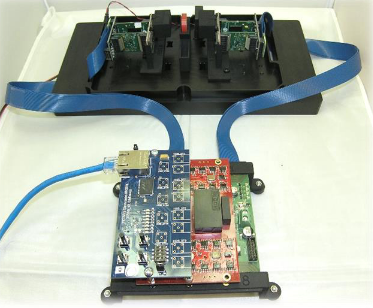
\includegraphics[scale=0.8]{3DesignPrinciples/32Tritium_detector/PETSYS_System.png}
\caption{Different parts of PETsys system\label{fig:PETSYS}~\cite{PETSYS}.}
\end{figure}
TRITIUM is a modular detector which sensitivity could be improved by adding more modules and, therefore, its readout electronics should be scalable. This requeriment is fulfilled by PETsys since it has an additional module, called Clock and Trigger, with which up to $16$ different PETsys basic boards can be read out in parallel. This gives to PETsys a capacity of reading up to 256 SiPM arrays. 

The PETsys software is based on C++ and Python scripts that drive the main tasks required, such as time coincidence options between SiPM arrays or energy discrimination. This software is open source, giving the possibility to modify the current scripts or to develop others with additional functions. PETsys has a time resolution better than $30~\pico\second$ which is one of the best time resolution of commercial systems available. Its price is around $10~\euro/$channel, which is cheaper than similar electronic systems. The PETsys system has the ability to monitor the temperature of the SiPM arrays and ASICS. In PETsys, the stabilization method of the SiPM gain, reported in section \ref{sec:CharacterizationSiPM}, can be implemented.

Some characterization measurements were carried out using the PETsys system to verify that the system works properly but the SiPM characterization was carried out at the level of a single channel (individual SiPM). The reason is that the output information of PETsys is already integrated and digitized, so it does not allow SiPM to be calibrated. Therefore, to characterize a SiPM, a PCB shown in Figure \ref{fig:PCBSiPM} was designed to bias the SiPM and to amplify its output signal. 

\begin{figure}
\centering
    \begin{subfigure}[b]{0.5\textwidth}
    \centering
    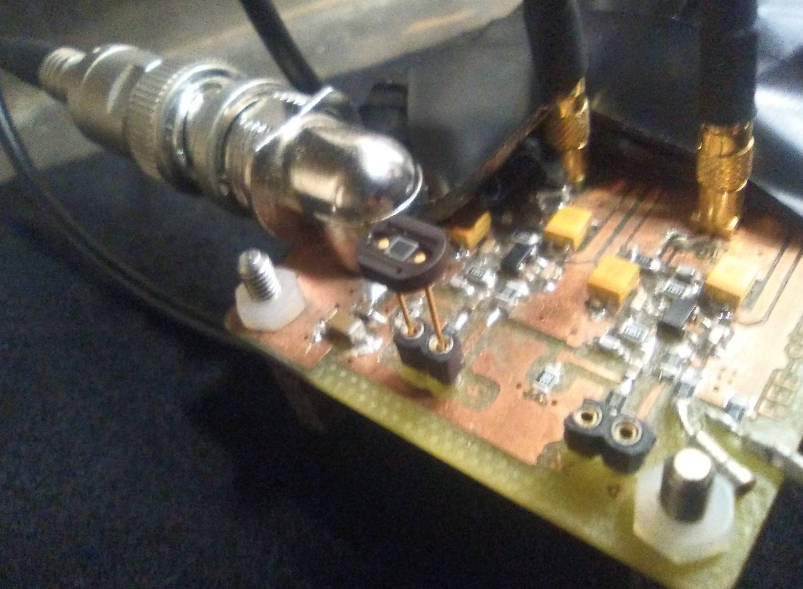
\includegraphics[width=\textwidth]{3DesignPrinciples/32Tritium_detector/SiPMPCB.png}  
    \caption{\label{subfig:ElectronicBoardSiPM}}
    \end{subfigure}
    \hfill
    \begin{subfigure}[b]{0.45\textwidth}
    \centering
    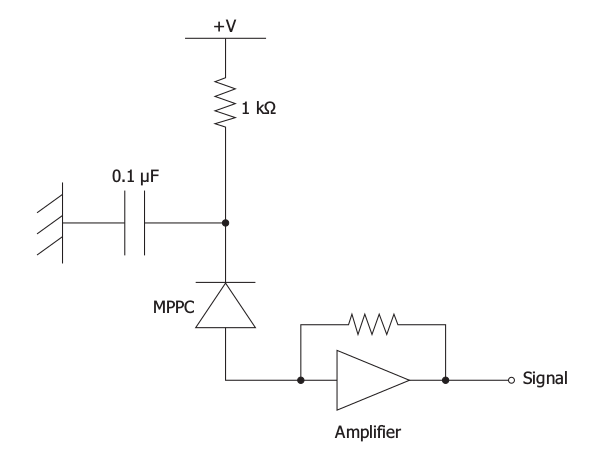
\includegraphics[width=\textwidth]{3DesignPrinciples/32Tritium_detector/ElectronicSchemePCBSiPM.png}  
    \caption{\label{subfig:ElectronicSchemePCBSiPM}}
    \end{subfigure}
    \hfill
 \caption{a) Electronic board used in the SiPM characterization. b) Electronic scheme on which this PCB is based.}
 \label{fig:PCBSiPM}
\end{figure}
This PCB was powered at $\pm6~\volt$ using a ISOTECH IPS-4303 voltage source \cite{VoltageSourceISOTECH} and the SiPM was biased by a KETHLEY 6517B electrometer \cite{VoltageSourceKethley}. The output signal was connected to a LeCroy WaveRunner 625Zi oscilloscope \cite{OscilloscopeIFIMED} that recorded the data which were subsequently analyzed using ROOT.